\documentclass{sig-alternate-05-2015}

% Do not include ISBN and DOI info
\makeatletter
\def\@copyrightspace{\relax}
\makeatother

\begin{document}
	
	\title{CS 211 course project proposal: \\Remote access to OpenWRT}
	
	\numberofauthors{3}
	
	\author{
		\alignauthor
		Zhehao Wang \\
               \affaddr{Department of Computer Science, UCLA}\\
		\email{zhehao@cs.ucla.edu}
		% 2nd. author
		\alignauthor
		Haitao Zhang \\
               \affaddr{Department of Computer Science, UCLA}\\
		\email{haitao@cs.ucla.edu}
		% 3rd. author
		\alignauthor 
		Jeffrey Chen\\
               \affaddr{Department of Computer Science, UCLA}\\
		\email{jc4556@g.ucla.edu}
	}
	
	\maketitle
	
	\section{Problem Statement}
	
	This project addresses remote access of an OpenWRT-based access point (AP) using Android mobile devices.

	OpenWRT is a free, open-source, Linux-kernel based operating system (OS) for network-routing embedded systems. This OS is notable for being able to run on various types of devices and for simplifying cross-platform building of OpenWRT software packages, including fixes for devices no longer supported by the devices' manufacturers.
	
	OpenWRT can be configured using a command-line interface or a web interface. The command-line interface is more suitable to professional users, while a web interface is more friendly to common users. However, OpenWRT's existing remote access web interface is not phone-friendly, being made for web browsers. On mobile smart devices, the in-browser interface is not scaled to the dimensions of the device's screen nor is it touch-friendly, hampering user comprehension and control of the interface. Certain mobile browsers may also impose limitations to file access, access that is necessary for configuration packages. Additionally, depending on the device, loss of connection or suspension of the browser to another application can force renewal of the session or prevent retrieval of network information, causing issues for presenting real-time data and visualizations.
	
	A native smart device application is more distribution-friendly for smart devices and can be designed on smart devices to be more user-friendly and streamlined to OpenWRT uses. Therefore, this project seeks to create a lightweight, easy-to-use generic Android application available for products running OpenWRT.
	
	\section{literature survey}
	
	\subsection{What is OpenWRT}
	OpenWRT \cite{fainelli2008OpenWRT, kim2014implementation} is a Busybox/Linux based embedded platform which is developed following GPL license. It minimizes its own functions so that it fits for lots of memory constrained devices. Specifically, it builds the appropriate toolchain for devices, compiles appropriate kernel with patched and options, as well as provides software as IPKG packages.
	
	\subsection{OpenWRT System Structure}
	OpenWRT System Structure covers four aspects: directory structure, packages and external repositories, toolchain, and software architecture.
	
	There are four key directories in the base: tools, toolchain, package and target.
	Tools and toolchain refer to common tools which will be used to build the firmware image, the compiler, and the C library.
	
	In OpenWRT, almost all the packages are .ipk files. Users can choose what packages to install and what packages to uninstall based on their specific needs. Packages are either part of the main trunk or maintained out of the main trunk. For the second case, packages can be maintained by the package feeds system.
	
	To compile the program for a particular architecture, the OpenWRT system will automatically create the toolchain during the cross-compilation process, simplifying the development tasks. However, if the toolchain needs to be created manually, OpenWRT also provides an easy way to configure the arguments.
	
	Figure \ref{OpenWRT:stack} shows the software stack of OpenWRT. We can see that the common embedded Linux tools such as uClibc, busybox, shell interpreter are used by OpenWRT.
	
	\begin{figure}
		\centering
		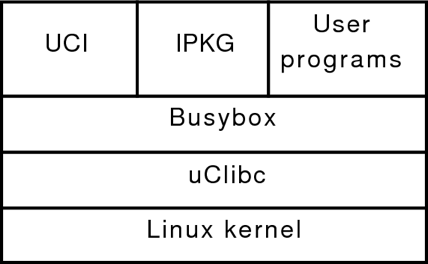
\includegraphics[width=0.4\textwidth]{stack.png}
		\caption{the software stack of OpenWRT}
		\label{OpenWRT:stack}
	\end{figure}
	
	\subsection{How to Develop With OpenWRT}
	
	It is easy to port software to OpenWRT. Various fetching methods such as GIT, Subversion, CVS, HTTP, local source can be used to download package source. In a typical package directory, there should always be a \verb|package/<name>/Makefile|. After running ``make menuconfig'', the new package will show up in the menu; and after running ``make'', the new package will be built.
	
	\subsection{Web-based Access to OpenWRT}
	In the OpenWRT system, some important features are provided: a built-in web server with CGI support, an SSH server and a package management tool. We can make use of these existing tools to build our Android application.
	
	Apart from the basic tools, OpenWRT also supports LuCI \cite{LuCI}, which is a browser-based tool to remotely configure the OpenWRT system. Specifically, it provides status visualization functions, system administration functions and network configurations. We would provide similar functions in our Android application.
	
	Another useful reference is the Netgear \cite{netgear} mobile application, which designs nice UIs that we can borrow ideas from. We need also to design the web-based access application UIs based on their work.
	
	\section{Design and implementation \\ roadmap}
	
	Based on the functional modules of LuCI, we will design the functional components of the Android application, which are organized into three major categories:
	
	\begin{itemize}
		
		\item
		\textbf{Network configuration} covers common functionalities in configuration tools that often come with commercial APs. These configurations include, but may not be limited to, managing network interfaces, DHCP and DNS settings, static routes, and firewall.
		
		\item
		\textbf{System configuration} provides an interface to customize the OpenWRT box. Common adminstration functions include: system and user configuration (setting device adminstrator password, creating system backup image and restoring system from backup image, generating user SSH keys, etc), software management (installing and configuring software packages) and task management (managing scheduled task and startup task). If the time allows, an in-application command line tool can be implemented for advanced users to execute console commands from the application to further customize the OpenWRT box.
		
		\item
		\textbf{Status/Statistics visualization} offers a mobile-phone friendly view of the system status (firmware and kernel version, uptime, current time; CPU and memory usage, currently running processes, system and kernel log) and network-related status (interface, route, firewall status, etc). The visualization component can provide real-time graphs of system load and traffic statistics, such as historical system memory usage, network traffic per interface and traffic per transport layer connection.
		
	\end{itemize}
	
	The design and implementation effort will be organized by the three function categories, with approximately one and a half weeks dedicated to each.
	
	\section{Timeline}
	
	A rough timeline for the project is given in table \ref{table:timeline}.
	
	\begin{table}[h]
		\centering
		\caption{Project timeline}
		\label{table:timeline}
		\begin{tabular}{p{3cm}|p{5cm}} \hline
			Week No. & Task \\ \hline
			5, 6 (first half) & Implement status/statistics visualization module \\ \hline
			6 (second half), 7 & Implement network configuration module \\ \hline
			8, 9 (first half) & Implement system administration module \\ \hline
			9 (second half), 10 & Prepare final report and presentation \\
			\hline\end{tabular}
	\end{table}
	
  \bibliographystyle{abbrv}
  \bibliography{proposal}

\end{document}